\documentclass[a4paper]{article}
\usepackage[utf8]{inputenc}
\usepackage[T2A]{fontenc}
\usepackage[12pt]{extsizes}

\usepackage[english,russian]{babel}
\usepackage[left=10mm, top=10mm, right=10mm, bottom=20mm, nohead, nofoot]{geometry}
\usepackage{amsmath,amsfonts,amssymb} % математический пакет
\headsep=10mm

\usepackage[most]{tcolorbox} % для управления цветом
% НАСТРОЙКИ
%теорема
\definecolor{theorem-color}{gray}{0.90} % уровень прозрачности (1 - максимум)
\newtcolorbox{htheorem}{colback=theorem-color,grow to right by=-4mm,grow to left by=-4mm,
    boxrule=0pt,boxsep=0pt,breakable} % настройки области с изменённым фоном

%определение
\definecolor{def-color}{gray}{0.98}
\newtcolorbox{definit}{colback=def-color,grow to right by=-4mm,grow to left by=-4mm,
    boxrule=0pt,boxsep=0pt,breakable} % настройки области с изменённым фоном

%доказательсвто теоремы
\definecolor{proof-color}{gray}{0.95} % уровень прозрачности (1 - максимум)
\newtcolorbox{hproof}{colback=proof-color,grow to right by=-1mm,grow to left by=-1mm,
    boxrule=0pt,boxsep=0pt,breakable} % настройки области с изменённым фоном

%замечания, следствия
\definecolor{consectary-color}{gray}{0.95} % уровень прозрачности (1 - максимум)
\newtcolorbox{cns}{colback=consectary-color,grow to right by=-4mm,grow to left by=-4mm,
    boxrule=0pt,boxsep=0pt,breakable} % настройки области с изменённым фоном



\usepackage{fancybox,fancyhdr}
\pagestyle{fancy}

\usepackage{hyperref}
\hypersetup{colorlinks=true, allcolors=[RGB]{010 090 200}} % цвет ссылок 
\newcommand{\lr}[1]{\left({#1}\right)} % команда для скобок

\author{Васильев Павел}
%\linespread{1}
\usepackage{amsmath}

\usepackage{graphicx}
\usepackage{ifpdf}
\ifpdf
\DeclareGraphicsRule{*}{mps}{*}{}
\fi
\usepackage{graphicx}
\usepackage{color}
\graphicspath{ {images/} }
%\renewcommand{\familydefault}{\sfdefault}

\begin{document}

\section*{Домашняя контрольная работа по матанализу 2}

\subsection*{1.$\displaystyle \lim_{n \rightarrow \infty} \sum_{k=1}^n \frac{\sqrt{k}}{n \sqrt{n} + k \sqrt{k}}$}

$\displaystyle \sum_{k=1}^n \frac{\sqrt{k}}{n \sqrt{n} + k \sqrt{k}} = \sum_{k=1}^n  \frac{1}{n} \frac{n \sqrt{k}}{n \sqrt{n} + k \sqrt{k}} = \frac{1}{n} \sum_{k=1}^n  \frac{\sqrt{k}}{\sqrt{n} + \frac{k \sqrt{k}}{n}} = \frac{1}{n}  \sum_{k=1}^n \frac{1}{\frac{\sqrt{n}}{\sqrt{k}} + \frac{k}{n}} = \frac{1}{n} \sum_{k=1}^n \frac{1}{ \left( \frac{k}{n} \right)^{-\frac{1}{2}} + \frac{k}{n}} = \frac{1}{n} \sum_{k=1}^n f \left( \frac{k}{n} \right)$

\[ \displaystyle f(x) = \frac{1}{x^{-\frac{1}{2}} + x} = \frac{ \sqrt{x} }{1 + x \sqrt{x}}
\]

\[
\displaystyle \lim_{n \rightarrow \infty} \frac{1}{n} \sum_{k=1}^n f \left(\frac{k}{n} \right) = \int_0^1 f(x) dx = \int_0^1 \frac{ \sqrt{x} }{1 + x \sqrt{x}} dx
\]

\[
\int \frac{ \sqrt{x} }{1 + x \sqrt{x}} dx = \begin{bmatrix}
t = \sqrt{x} \\
 dt = \frac{dx}{2t}
\end{bmatrix}
= \int \frac{2t^2}{1+t^3} dt = 2 \left( \int \frac{1}{3(t+1)} dt + \int \frac{2t-1}{3(1-t+t^2)} dt \right) =
\]

\[
= 2 \left( \frac{1}{3} \ln |t+1| +\int \frac{2t-1}{3(1-t+t^2)} dt \right) = \begin{bmatrix}
u = 1-t+t^2 \\ du = (2t-1)dt
\end{bmatrix} = 2 \left( \frac{1}{3} \ln |t+1| + \frac{1}{3} \ln|u| \right) =
\]

\[
= \frac{2}{3} \left(\ln |t+1| + \ln|1-t+t^2| \right) + C = 
\]

\[
= \frac{2}{3} \left( \ln |\sqrt{x}+1| + \ln|1-\sqrt{x}+x| \right) + C
\]

\[
\int_0^1 f(x)dx = \frac{2}{3} \left( \ln |\sqrt{x}+1| + \ln|1-\sqrt{x}+x| \right) \bigg|_0^1 = \frac{2}{3} \left( \ln 2 + \ln 1 - \ln 1 - \ln 1 \right) = \frac{2 \ln 2}{3}
\]

\textit{Ответ: $\frac{2 \ln 2}{3}$}


\subsection*{2. $y = \sqrt{4-x^2}, y=0, 0 \leq x \leq 1$}

\[ \int \sqrt{4-x^2} dx  = \begin{bmatrix}
x = 2\sin t \\ dx = 2 \cos t dt \\ t = \arcsin(\frac{x}{2})
\end{bmatrix} = 2 \int \cos^2 t dt = 4 \int \frac{1+\cos 2t}{2} dt = \sin 2t + 2t + C =
\] 

\[ = \sin \left( 2 \arcsin \left( \frac{x}{2}\right) \right) + 2 \arcsin \left( \frac{x}{2} \right) + C\]

\[\int_0^1 \sqrt{4-x^2} dx  =
\left( \sin \left( 2 \arcsin \left( \frac{x}{2}\right) \right) + 2 \arcsin \left( \frac{x}{2} \right) \right) \bigg|_0^1 = \]

\[ =  \left( 2 \sin \left( \arcsin \left( \frac{x}{2} \right) \right) \cos \left( \arcsin \left( \frac{x}{2}\right) \right) + 2 \arcsin \left( \frac{x}{2} \right) \right) \bigg|_0^1 = 
\]

\[
= \left( 2 \frac{x}{2} \sqrt{1-\frac{x^2}{4}} + 2 \arcsin \left( \frac{x}{2} \right) \right) \bigg|_0^1
= \left( \frac{x}{2} \sqrt{4-x^2} + 2 \arcsin \left( \frac{x}{2} \right) \right) \bigg|_0^1
=
\]

\[
=
\frac{\sqrt{3}}{2} + 2 \arcsin \left( \frac{1}{2} \right) = \frac{\sqrt{3}}{2} + \frac{\pi}{3}
\]

\textit{Ответ:$\frac{\sqrt{3}}{2} + \frac{\pi}{3}$}

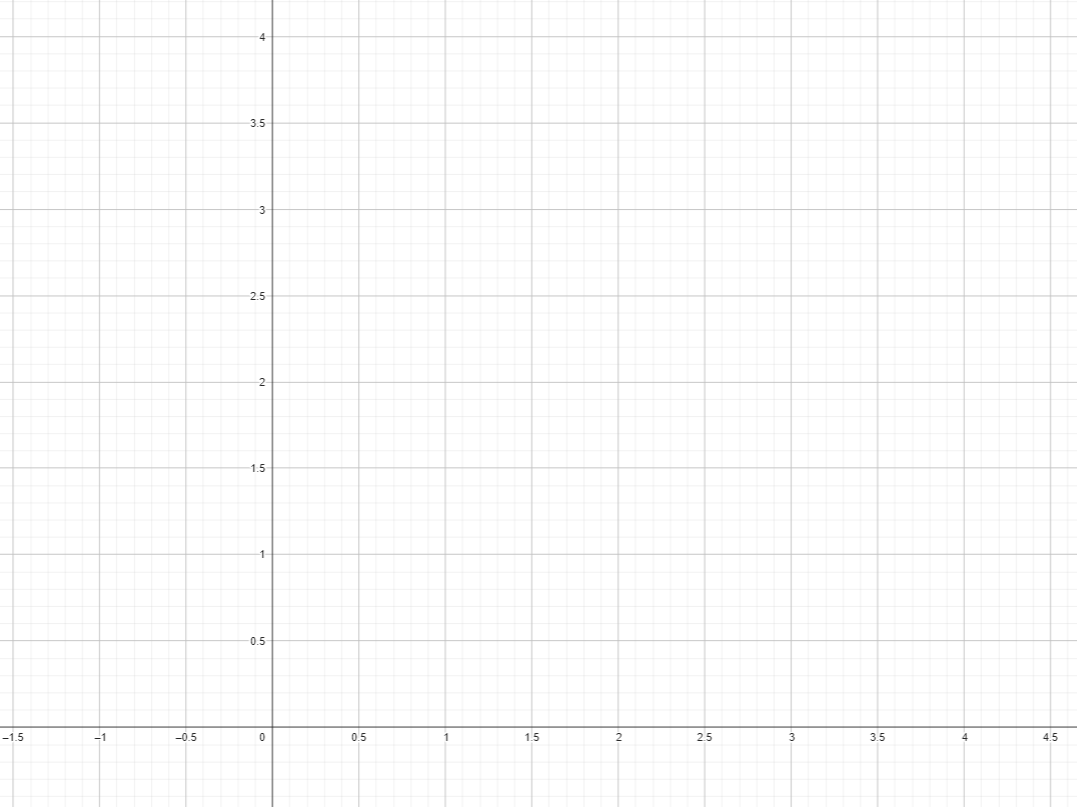
\includegraphics[width=18cm]{graphic.png}

\subsection*{3. $\begin{cases} x(t) = 4( \cos t + t \sin t) \\ y(t) = 4 ( \sin t - t \cos t) \end{cases} 0 \leq t \leq 2 \pi$}

\[L = \left( x(t), y(t) \right)\]
\[|L| = \int_0^{2 \pi} \sqrt{(x'(t))^2 + (y'(t))^2} dt\]


\[ x'(t) = 4(- \sin t + \sin t + t \cos t) = 4 t \cos t\]

\[ y'(t) = 4(\cos t - \cos t + t \sin t) = 4 t \sin t\]

\[ |L| = \int_0^{2 \pi} \sqrt{(4t)^2 (\sin^2 t + \cos^2 t)} dt = \int _0^{2 \pi} 4t dt = 2t^2 \bigg|_0^{2 \pi} = 8 \pi^2 \]

\textit{Ответ: $8 \pi^2$}

\subsection*{4. $\displaystyle \int_0^{\arctan \left( \frac{1}{3} \right)} \frac{8+\tan x}{18 \sin^2 x + 2 \cos^2 x} dx$}

\[ 
I = \int_0^{\arctan \left( \frac{1}{3} \right)} \frac{8+\tan x}{18 \sin^2 x + 2 \cos^2 x} dx = \begin{bmatrix}
t = \tan x \\ dt = \frac{dx}{\cos^2 x}
\end{bmatrix} = \int_0^{\frac{1}{3}} \frac{8+t}{18t^2+2}dt \]

\[ \int \frac{8+t}{18t^2+2}dt = \frac{1}{2} \int \frac{8+t}{9t^2+1} dt = \]
 \[ =\frac{1}{2} \left( \int \frac{8}{9t^2+1} dt + \int \frac{t}{9t^2 + 1} dt \right) = \frac{1}{2} (I_1 + I_2)
\]

\[ I_1 =  \int \frac{8}{9t^2+1} dt = \begin{bmatrix}
u = 3t \\ du = 3dt
\end{bmatrix} = \frac{1}{3} \int \frac{8}{u^2+1} du = \frac{8}{3} \arctan(3t) \]

\[ I_2 =  \int \frac{t}{9t^2 + 1} dt = \begin{bmatrix}
u = 9t^2+1 \\ du = 18t dt
\end{bmatrix} = \frac{1}{18} \int \frac{du}{u} = \frac{\ln|u|}{18} = \frac{\ln(9t^2+1)}{18} \]

\[ I = \frac{1}{2} \left( \frac{8}{3} \arctan (3t) + \frac{1}{18} \ln (9t^2 + 1) \right) \bigg|_0^{\frac{1}{3}} = \frac{1}{2} \left( \frac{8}{3} \frac{\pi}{4} + \frac{1}{18} \ln 2 \right) = \frac{\pi}{3} + \frac{\ln 2}{36} \]

\textit{Ответ: $\frac{\pi}{3} + \frac{\ln 2}{36}$}


\subsection*{5. $\displaystyle \lim_{\varepsilon \rightarrow +0} \int_{\frac{\varepsilon}{2}}^{\ln (1+\varepsilon)} \frac{1}{x} \arctan \frac{x+1}{\sin x} dx$}

$\Phi(x) =\frac{1}{x}$ - положительная функция на отрезке $[\frac{\varepsilon}{2}; \ln (1+\varepsilon)]$,
$f(x) = \arctan \frac{x+1}{\sin x}$ - непрерывная на этом же отрезке при достаточно малом $\varepsilon$.
 
Тогда при достаточно малых $\varepsilon$ справедлива теорема о среднем и тогда исходный интеграл под знаком предела равен \[\mu \int_{\frac{\varepsilon}{2}}^{\ln (1+\varepsilon)} \frac{1}{x} dx\] где $\mu \in [\min f, \max f]$.

Найдём $\min f$ и $\max f$:

\[
\left( \arctan \frac{x+1}{\sin x} \right)' = \frac{\left(\frac{x+1}{\sin x}\right)'}{1+\left( \frac{x+1}{\sin x} \right)^2} =  \frac{\sin x - (x+1) \cos x}{1+\left( \frac{x+1}{\sin x} \right)^2}
\]

Посмотрим на $\sin x - (x+1) \cos x$. При достаточно малых $\varepsilon$, например, меньше, чем $\frac{\pi}{3}$ имеем $\sin x < \frac{1}{2}$, $\cos x > \frac{\sqrt{3}}{2}$, $x+1>1$.
Поэтому 

\[
\sin x - (x+1) \cos x < \frac{1}{2} - \frac{\sqrt{3}}{2} < 0
\]

Значит $\max f = f \left( \frac{\varepsilon}{2} \right), \min f = f \left( \ln (1+ \varepsilon) \right)$.

Устремляя $\varepsilon$ к нулю и учитывая, что $\mu \in \left[ f \left( \ln (1+ \varepsilon) \right), f \left( \frac{\varepsilon}{2} \right) \right]$ и то, что $\ln (1 + \varepsilon)$ и $\frac{\varepsilon}{2}$ стремятся к нулю, получаем (по лемме о двух милиционерах), что  

\[\mu = 
\lim_{\varepsilon \rightarrow 0} \arctan \frac{\varepsilon+1}{\sin \varepsilon} = \arctan \left( \lim_{\varepsilon \rightarrow 0} \frac{\varepsilon+1}{\sin \varepsilon} \right) = \frac{\pi}{2}\]

\[\displaystyle \lim_{\varepsilon \rightarrow +0} \int_{\frac{\varepsilon}{2}}^{\ln (1+\varepsilon)} \frac{1}{x} \arctan \frac{x+1}{\sin x} dx = \lim_{\varepsilon \rightarrow +0}  \frac{\pi}{2} \int_{\frac{\varepsilon}{2}}^{\ln (1+\varepsilon)} \frac{1}{x} dx = \lim_{\varepsilon \rightarrow +0} \frac{\pi}{2} \left( \ln x \right) \bigg|_{\frac{\varepsilon}{2}}^{\ln (1+\varepsilon)} = 
\]

\[
= \lim_{\varepsilon \rightarrow +0} \frac{\pi}{2}\left( \ln \left( \ln (1+ \varepsilon) \right) - \ln \left( \frac{\varepsilon}{2} \right) \right) = \lim_{\varepsilon \rightarrow +0} \frac{\pi}{2}\left( \ln \left( \frac{\ln (1+\varepsilon)}{\frac{\varepsilon}{2}} \right) \right) = \frac{\pi}{2} \ln 2
\]

\textit{Ответ: $ \frac{\pi}{2} \ln 2$}
\end{document}
